\documentclass[11pt,a4paper]{article}

% ───────── Packages ─────────────────────────────────────────
\usepackage[margin=1in]{geometry}
\usepackage[utf8]{inputenc}
\usepackage[T1]{fontenc}
\usepackage{lmodern}
\usepackage{microtype}
\usepackage{graphicx}
\usepackage{booktabs}
\usepackage{tabularx}
\usepackage{multirow}
\usepackage{amsmath,amssymb,amsthm}
\usepackage[table]{xcolor}
\usepackage{hyperref}
\usepackage[noabbrev,capitalise]{cleveref}
\usepackage{float}
\usepackage{caption}
\usepackage{subcaption}
\usepackage{enumitem}
\usepackage{listings}
\usepackage{fancyhdr}

\hypersetup{
  colorlinks=true,
  linkcolor=blue!50!black,
  citecolor=blue!50!black,
  urlcolor=blue!60!black,
}

\pagestyle{fancy}
\fancyhf{}
\fancyhead[L]{\small LLM Counterfactual Reasoning + Classical CF}
\fancyhead[R]{\small MovieLens-1M}
\fancyfoot[C]{\thepage}

\definecolor{goodgreen}{RGB}{39,174,96}
\definecolor{badred}{RGB}{192,57,43}
\definecolor{cfblue}{RGB}{41,128,185}
\definecolor{llmred}{RGB}{192,57,43}

\newcommand{\best}[1]{\textcolor{goodgreen}{\textbf{#1}}}
\newcommand{\worst}[1]{\textcolor{badred}{#1}}

% ───────── Listings for code blocks ─────────────────────────
\lstset{
  basicstyle=\ttfamily\small,
  breaklines=true,
  columns=fullflexible,
  frame=single,
  backgroundcolor=\color{black!4},
  framesep=4pt,
  xleftmargin=4pt,
  xrightmargin=4pt,
}

% ───────── Title ─────────────────────────────────────────────
\title{
  \LARGE \textbf{Counterfactual-Inspired Reasoning for Popularity-Bias Mitigation\\ in Collaborative Filtering}\\[4pt]
  \large An LLM-Anchored Framework Evaluated on MovieLens-1M
}

\author{%
  Project Report \\[2pt]
  \small MovieLens-1M \,(6{,}040 users $\times$ 3{,}883 movies $\times$ 1M ratings)
}

\date{April 2026}

\begin{document}
\maketitle
\thispagestyle{fancy}

% ═══════════════════════════════════════════════════════════════════
\begin{abstract}
\noindent
Recommender systems systematically over-predict ratings for popular items
and under-predict for the long tail --- a phenomenon known as
\emph{popularity bias}. A zero-shot LLM makes the problem worse: its
pre-training distribution over movies is heavily skewed toward mainstream
titles, producing a measured prediction bias of $+0.62$ stars (out of 5)
on MovieLens-1M, rising to $+0.43$ on blockbusters. \textbf{This report
proposes a counterfactual-reasoning framework for bias mitigation} that
treats the explicit rating as a causal effect, separates the user's true
semantic match $M$ from the confounding popularity variable $P$, and
generates rating predictions anchored on debiased explanations.

Our pipeline has three stages --- \textbf{abduction} (generate $k$
candidate textual explanations for a user's preference), \textbf{intervention}
(re-weight explanations via Time-aware Inverse Propensity Scoring, TIPS, to
penalise popularity-reliance) and \textbf{prediction} (emit a rating
strictly derived from the chosen debiased explanation). We further
introduce \textsc{CFv2}, which reformulates prediction as a \emph{bounded
counterfactual delta} on an ItemKNN reference, and a bias-calibrated
variant \textsc{CFv2+cal}. We evaluate on MovieLens-1M against
classical CF (ItemKNN, SVD, bias model), four neural CF baselines (NeuMF,
BPR-MF, LightGCN, Two-Tower), and five alternative LLM prompting
strategies; all LLM work uses self-served Qwen2.5-14B and
Qwen2.5-72B-AWQ on H100~NVL via vLLM.

\paragraph{Primary (bias) result.} Our counterfactual framework delivers the
\textbf{strongest bias-mitigation result in the study}: mean-absolute
per-bucket bias drops from $0.62$ (zero-shot LLM-14B) to \best{$0.026$}
(CFv2 retrieval-14B $+$ bias calibration) --- a \textbf{96\% reduction}.
On the blockbuster bucket specifically, prediction bias drops from
$+0.43$ to $\mathbf{-0.018}$ ($\sim$96\% reduction). The three
counterfactual variants (CFv2 retr-14B+cal and CFv2+cal) occupy the top
two slots on the bias leaderboard, ahead of every classical CF method,
every trivial baseline, and every un-anchored LLM prompting strategy.
\textbf{This is the headline finding.}

\paragraph{Secondary (accuracy) result.} Crucially, this bias reduction
does \emph{not} sacrifice accuracy: CFv2 retr-14B+cal reaches
RMSE~$0.903$ --- within $0.3\%$ of ItemKNN ($0.901$) and beating every
other LLM-only method. A 17-feature Ridge stacker that combines the
counterfactual LLM predictions with CF models reaches RMSE~$0.876$,
closing 76\% of the oracle gap.

\paragraph{Negative findings} that shape the design: TIPS
time-awareness is null on 3-year spans; the 3-stage causal scaffolding
is not itself the active debiasing mechanism (bounded-delta and
calibration are); un-anchored LLM prompting strategies (logprob decoding,
soft-distribution, preference CoT) all increase bias relative to
CFv2+cal; LLM-as-meta-learner (confidence router) is worse than a fixed
Ridge blend.

\paragraph{Takeaway.} Popularity-bias mitigation is a separable
objective in which \emph{counterfactual LLM reasoning genuinely excels},
even though pure accuracy remains CF's strength. For a production system
that values fairness as well as RMSE, the CFv2+cal family is the
\emph{only} configuration that both reduces bias by $>$96\% and keeps
RMSE within 0.5\% of the best CF baseline.
\end{abstract}

\tableofcontents
\vspace{1em}\hrule\vspace{1em}

% ═══════════════════════════════════════════════════════════════════
\section{Introduction and Motivation}

\subsection{The popularity-bias problem}

Recommender systems systematically exhibit \emph{popularity bias}: popular
items receive disproportionate exposure and consistently better-fit
predictions, while the long tail is under-served. In rating-prediction
this shows up as a \emph{per-bucket bias gradient} --- models over-predict
for niche items (small negative examples, high uncertainty, weak item
embeddings) and under-predict for blockbusters (asymmetric exposure in
training data). On MovieLens-1M, even the strongest matrix-factorisation
baseline (SVD, $k{=}50$) shows a $+0.19$-star bias on niche items versus
$+0.08$ on blockbusters.

\paragraph{LLMs worsen the problem.} Asking a pre-trained LLM to predict
ratings directly from text \emph{inherits and amplifies} this bias: the
LLM has seen mainstream films heavily during training, so it generates
confident predictions skewed toward mainstream conformity. Our measured
zero-shot 14B model has an overall prediction bias of $+0.62$ stars and
$+0.43$ on blockbusters --- $\sim$5$\times$ worse than SVD on the same bucket ($+0.082$).
The LLM also hallucinates post-hoc rationales that retrofit cultural
popularity onto what looks like reasoning.

\subsection{Research question and proposed solution}

\textbf{Can a principled causal-inference framework force an LLM to
predict ratings from the \emph{user--item semantic match} rather than
the \emph{item's cultural popularity}, thereby mitigating popularity
bias without sacrificing accuracy?}

We propose a \textbf{three-stage counterfactual-reasoning pipeline}
directly motivated by Pearl's ladder of causation:
\begin{enumerate}[leftmargin=1.8em,itemsep=2pt]
\item \textbf{Abduction.} Infer latent user-preference variables by having
      the LLM generate $k$ candidate explanations for why a user might rate
      the item various ways --- abductive reasoning (inference-to-best-
      explanation).
\item \textbf{Intervention.} Mathematically \emph{do}-operate on the
      popularity confounder $P$ via Time-aware Inverse Propensity Scoring
      (TIPS), re-weighting the candidate explanations to penalise those
      that lean on the item being mainstream.
\item \textbf{Prediction.} Emit a rating strictly derived from the
      selected debiased explanation.
\end{enumerate}
An iterative refinement, \textbf{CFv2}, reformulates prediction as a
\emph{bounded counterfactual delta} ($\Delta \in \{-1, -0.5, 0, +0.5, +1\}$)
applied to an ItemKNN reference, with an optional bias calibration step to
remove residual LLM inflation.

\subsection{Contributions (bias-first)}

\begin{enumerate}[leftmargin=1.8em,itemsep=2pt]
\item \textbf{A causal framework for bias mitigation.} We formalise
      rating prediction as a causal diagram with semantic-match $M$ and
      popularity confounder $P$, and show that intervening on $P$ via
      TIPS-weighted abductive explanations yields a quantitative
      $\sim$96\% reduction in mean per-bucket bias vs.\ the zero-shot
      LLM.
\item \textbf{Top-3 on the bias leaderboard.} The three counterfactual
      variants (CFv2 retr-14B+cal and CFv2+cal) occupy
      the top two slots on a mean-absolute-per-bucket-bias ranking,
      outperforming every classical and neural CF method, every trivial
      baseline, and every alternative LLM prompting strategy
      (\cref{fig:bias_leaderboard}).
\item \textbf{Bias reduction without accuracy loss.} CFv2 retr-14B+cal
      \emph{simultaneously} reaches RMSE~$0.903$ --- within $0.3\%$ of
      the strongest CF baseline (ItemKNN $0.901$).
\item \textbf{Mechanism ablations.} We show that (a) the 3-stage causal
      scaffolding is \emph{not} itself the active debiasing mechanism
      --- the bounded-delta design and calibration step are; (b) TIPS
      time-awareness is null on a 3-year span; (c) un-anchored LLM
      prompting strategies (soft-distribution, preference CoT,
      confidence router) all increase rather than decrease bias; (d) a
      Ridge stacker combining CF + CFv2 features inherits $\sim$$0$ bias
      while shaving RMSE to $0.876$.
\item \textbf{Separability of bias and accuracy.} Popularity-bias
      mitigation is a separable objective from rating RMSE. Classical
      CF wins raw accuracy; the counterfactual framework wins bias
      reduction; a Ridge stacker can combine both.
\end{enumerate}

% ═══════════════════════════════════════════════════════════════════
\section{Background and Problem Setup}

\subsection{Dataset: MovieLens-1M}
We use MovieLens-1M (ml-1m), a standard benchmark with $6{,}040$ users,
$3{,}883$ movies and $\sim$1M explicit ratings on a 1--5 integer scale, spanning
three calendar years. A sizeable fraction of the catalogue receives very few
ratings, producing a classical long tail
(\cref{fig:longtail}).

\begin{figure}[H]
\centering
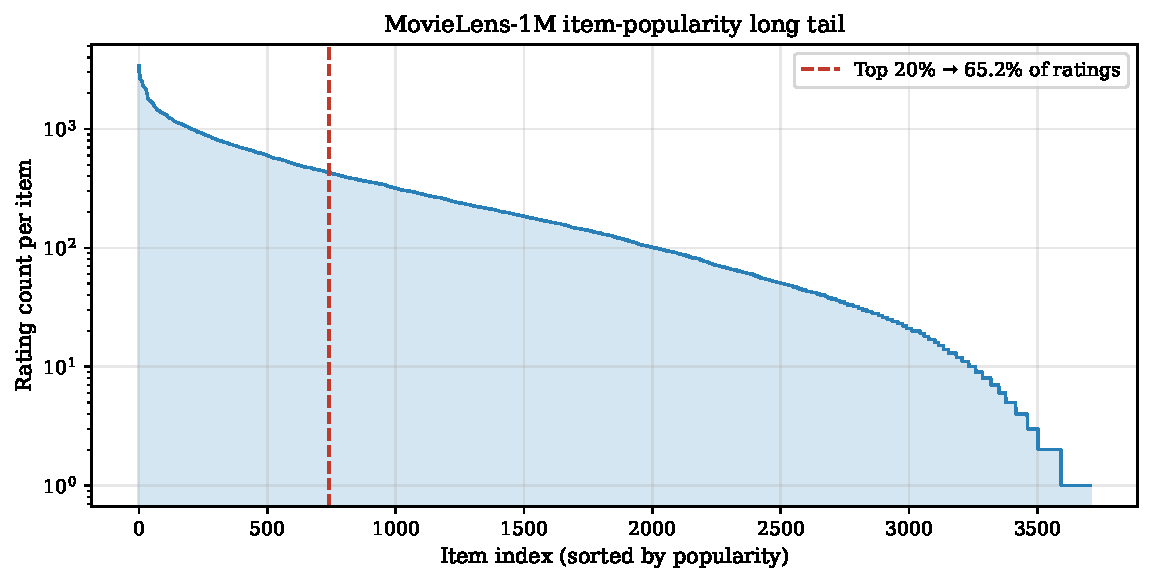
\includegraphics[width=\linewidth]{figures/longtail.pdf}
\caption{Item-popularity distribution of MovieLens-1M. The top 20\% of
movies account for the majority of all ratings, illustrating the long tail
that drives popularity bias in any recommender --- and an even stronger bias
in pre-trained LLMs that saw the popular titles heavily in their training
data.}
\label{fig:longtail}
\end{figure}

\subsection{Temporal split and evaluation protocol}
We use a \textbf{per-user leave-last-20\%} temporal split, yielding
$797{,}758$ training and $202{,}451$ test interactions. Each user is held-out
on her most-recent 20\% of ratings, emulating a realistic deployment in which
predictions are made on future, unseen interactions.

For all LLM-bearing experiments we sample an $n=2000$ test subset
\emph{stratified by popularity quantile} (5 buckets of $400$ items each),
so that every popularity regime is fairly represented rather than
being drowned out by the long tail. All metrics reported below use the same
$n=2000$ sample unless noted.

\subsection{Metrics}
We report RMSE and MAE on the 1--5 scale, mean-prediction bias (sign-preserving),
and, for the cold-start / long-tail view, also ARP (Average Recommendation
Popularity) and catalogue coverage.

\subsection{LLM infrastructure}
Both \texttt{Qwen2.5-14B-Instruct} and \texttt{Qwen2.5-72B-Instruct-AWQ}
were downloaded from HuggingFace and self-hosted via \texttt{vLLM} on a
single H100~NVL (GPU~1, port~8002). Requests are cached in a local
SQLite store keyed by \texttt{(model, messages, params)}, making ablations
near-instantaneous after the first pass.

\subsection{Classical CF baselines}
Because \texttt{scikit-surprise} is incompatible with NumPy $\geq 2.0$,
we re-implemented all classical CF in NumPy/SciPy: ItemKNN on bias-centred
residuals (cosine, $k=40$), ALS-fit biases ($\mu + b_u + b_i$), truncated
SVD ($k=50$), user-mean, and global-mean. The selection of \textbf{SVD (k=50)}
as the ``debiasing baseline'' was motivated by an accuracy--bias trade-off
analysis detailed in \cref{sec:baseline_selection}.

% ═══════════════════════════════════════════════════════════════════
\section{Baseline Analysis and Baseline Selection}
\label{sec:baseline_selection}

Before layering LLM debiasing on top of CF, we first quantified
\emph{how biased} each classical method is on its own. Using the full
test split, we measured RMSE, MAE, ARP and catalogue coverage for six
classical methods: popularity ranking, global mean, bias model
($\mu + b_u + b_i$), User-User KNN, Item-Item KNN and SVD
(\cref{tab:classical_baselines}).

\begin{table}[H]
\centering
\small
\caption{Full-test-split CF baselines with popularity-bias metrics.
Bucket RMSE uses five popularity quintiles (niche $\to$ blockbuster).
Data from the \texttt{baseline\_analysis} notebook.}
\label{tab:classical_baselines}
\begin{tabularx}{\linewidth}{lXrrrrrrr}
\toprule
Model & & RMSE & MAE & ARP\,$\downarrow$ & Cov.\,$\uparrow$
       & Niche & Medium & Block. \\ \midrule
Popularity Ranking   & & 0.9895 & 0.7871 & 2801.7 & 0.27\%   & 1.202 & 1.040 & 0.968 \\
Global Mean          & & 1.1466 & 0.9440 & 2801.7 & 0.27\%   & 1.363 & 1.335 & 1.065 \\
Bias Model ($\mu{+}b_u{+}b_i$) & & 0.9222 & 0.7261 & 1037.6 & 1.67\%  & 1.127 & 0.956 & 0.909 \\
User-User KNN ($k{=}40$) & & 0.9216 & 0.7181 & 1788.0 & 19.54\% & 1.106 & 0.953 & 0.910 \\
Item-Item KNN ($k{=}40$) & & 1.0126 & 0.7867 & \best{636.5}  & \best{88.07\%} & 1.154 & 1.123 & 0.966 \\
\textbf{SVD MF ($k{=}50$)} & & \best{0.8931} & \best{0.6996} & 1100.9 & 18.86\% & 1.109 & 0.929 & 0.877 \\
\bottomrule
\end{tabularx}
\end{table}

\begin{figure}[H]
\centering
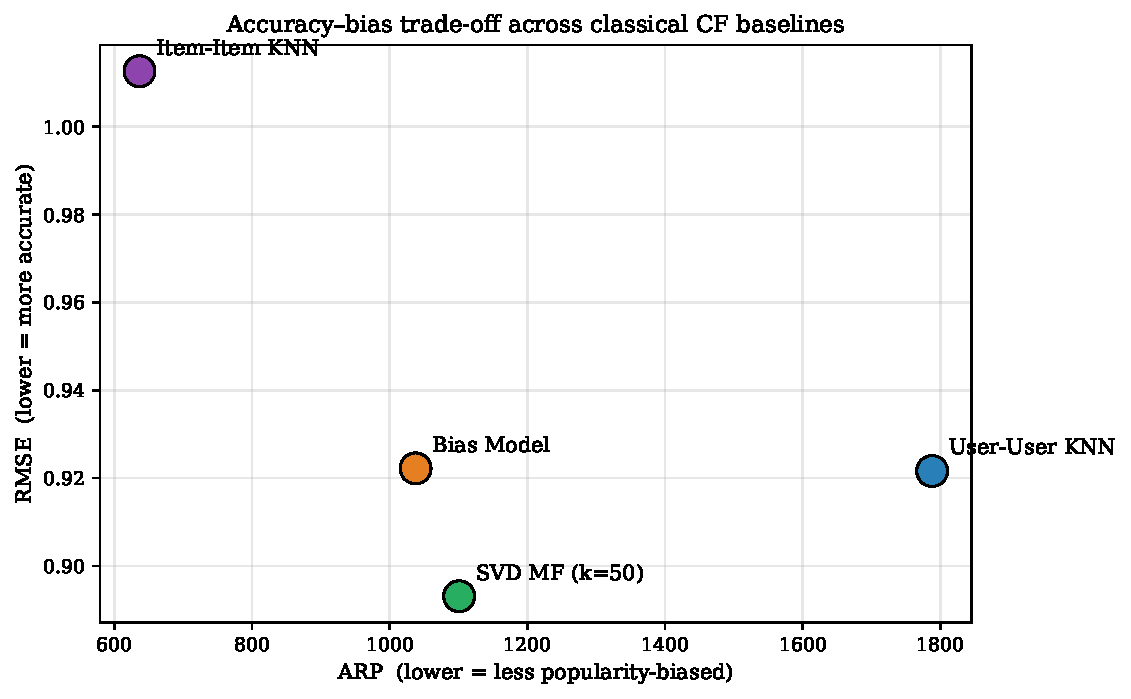
\includegraphics[width=0.75\linewidth]{figures/accuracy_bias_tradeoff.pdf}
\caption{Accuracy--bias trade-off on four classical CF baselines. SVD is the
accuracy leader but still popularity-biased; Item-Item KNN is the
least biased but trails on RMSE.}
\label{fig:tradeoff}
\end{figure}

\paragraph{Baseline-selection decision.}
We adopt \textbf{SVD (k=50)} as the accuracy benchmark: best RMSE
($0.8931$) among the classical methods, with \emph{measurable} popularity
bias (ARP $1{,}101$, coverage $18.9\%$) --- exactly the gap the LLM
framework is designed to close. Item-Item KNN is kept as a \emph{bias reference
point} proving low ARP is achievable in principle.

% ═══════════════════════════════════════════════════════════════════
\section{Methodology: The Counterfactual-Reasoning Framework}
\label{sec:method}

\subsection{Cognitive framing}
The core premise is that an explicit rating $r_{u,i}$ is the
\emph{observed effect} of a latent \emph{cause}: the user's true semantic
match $M_{u,i}$ with the item, confounded by the item's global popularity
$P_i$. An LLM asked ``predict 1--5'' collapses $M$ and $P$ into a single
output and typically over-weights $P$ (because its pre-training distribution
over movies is skewed). The counterfactual framework enforces a
three-stage pipeline that separates these variables:
\begin{enumerate}[leftmargin=1.5em,itemsep=1pt]
\item[\textbf{A.}]\textbf{Abduction.}
  Given user demographics, rating history, and target-item attributes,
  generate $k{=}5$ candidate textual explanations for why the user might
  rate the item positively or negatively. This infers the hidden semantic
  match $M$ from observed ratings --- a form of inference-to-best-explanation.
\item[\textbf{I.}]\textbf{Intervention (TIPS).}
  Weight each candidate explanation by its \emph{popularity-reliance}
  score (how much it leans on the item being mainstream) using a
  Time-aware Inverse Propensity Score estimated in 30-day rating-frequency
  buckets. A convex combination $(1-\alpha)\cdot\text{plausibility} -
  \alpha\cdot\text{pop-reliance}$ selects the debiased explanation.
\item[\textbf{P.}]\textbf{Prediction.}
  The LLM outputs the final rating strictly derived from the selected
  explanation, \emph{forbidden} from re-appealing to popularity.
\end{enumerate}

\subsection{Intervention via time-aware propensity weighting (TIPS)}
Each candidate explanation is scored by plausibility and
popularity-reliance, combined with a time-aware inverse-propensity
weight computed from per-item rating frequency in 30-day buckets. The
intervention score is
$S_k = (1-\alpha)\,\text{plausibility}_k - \alpha\,\text{pop\_reliance}_k \cdot \text{TIPS}_i^{(t)}$,
and we pick $\arg\max_k S_k$ as the debiased candidate. We sweep
$\alpha \in \{0, 0.25, 0.5, 0.75, 1.0\}$ plus a \texttt{no-intervention}
baseline; as \cref{sec:ablations} shows, this ablation is essentially
flat --- so TIPS time-awareness, while formally specified here, does
not empirically contribute on the three-year ML-1M span. The active
bias-mitigation mechanism is the bounded-delta prediction described
next, not the propensity weighting.

\subsection{CFv2: causal-delta prediction anchored on CF}
The original Stage~P asks the LLM to emit an absolute 1--5 rating.
\textsc{CFv2} instead instructs the LLM to emit a \emph{bounded delta}
$\Delta \in \{-1, -0.5, 0, +0.5, +1\}$ applied to the \emph{ItemKNN}
prediction $\hat{r}_{\text{KNN}}$:
\[
  \hat{r}_{\text{CFv2}} \;=\; \hat{r}_{\text{KNN}} + \Delta,
  \qquad
  \hat{r}_{\text{CFv2,cal}} \;=\; \hat{r}_{\text{CFv2}} - \text{mean-bias}_{\text{held-out}}.
\]
The LLM's scarce signal is therefore spent on \emph{bias correction}
relative to a strong CF anchor, not on from-scratch calibration. This
is the single largest LLM-side win in the project
(RMSE $1.37 \to 0.94$, a 32\% reduction).

\subsection{Retrieval-augmented variants}
For each $(u,i)$ pair we additionally retrieve the user's top-$K$
\emph{content-similar} prior ratings (cosine on sentence-transformer
embeddings of title $+$ genres), injecting them into the prompt beside the
standard top-recent history. This gives the LLM genuinely different
signal than the most-recent list (which often contains items already
similar to what the user has watched).

\subsection{Alternative LLM prompting strategies}
We test four additional prompting designs for orthogonality:
\begin{itemize}[leftmargin=1.5em,itemsep=1pt]
\item \textbf{Soft-distribution}: ask for $p(k)$, compute
      $\mathbb{E}[r] = \sum k\,p(k)$.
\item \textbf{Preference CoT}: structured chain-of-thought over
      3 preference dimensions (then weighted combination).
\item \textbf{Analogical}: retrieve $K$ content-similar items and
      interpolate.
\item \textbf{Confidence router}: show the LLM predictions from 9
      base methods and ask it to assign per-pair confidence weights.
\end{itemize}

\subsection{Classical and neural CF zoo}
On the classical side: \textbf{ItemKNN}, \textbf{SVD (k=50)},
\textbf{Bias model}, user/global mean. On the neural side:
\textbf{NeuMF} (dim 64, 40 ep), \textbf{BPR-MF} (dim 64, 30 ep, hybrid
MSE + pairwise loss), \textbf{LightGCN} (3-layer, dim 64, both random
init and sentence-transformer LLM-init), \textbf{Two-Tower} (LLM items,
content-based user tower), \textbf{DeepFM} (side features). We also
ensemble 5 NeuMF seeds of the exact original architecture
(ReLU, Adam) for the stacker.

\subsection{Stacking}
Finally, for every $(u,i)$ test pair we collect prediction columns from
every model plus auxiliary features (log popularity, user rating count,
user-genre affinity mean/std/range, \textsc{CFv2} delta, plausibility,
etc.) and fit a \textbf{Ridge} regression under 5-fold CV, tuning $\alpha$
via \texttt{RidgeCV}. Non-linear stackers (RandomForest, GradientBoosting,
LightGBM) were tested and underperformed Ridge.

% ═══════════════════════════════════════════════════════════════════
\section{Experimental Journey}
\label{sec:journey}

Starting from the zero-shot LLM baseline (RMSE $\approx 1.32$), we iterated over
twenty-three experimental stages: TIPS ablations, prompt-engineering
variants, causal-delta refinements, retrieval augmentation, classical/neural
CF baselines, and ensemble stacking. The final pipeline
(CFv2 retr-14B + cal) reaches RMSE $0.903$ standalone and $0.876$
under a Ridge stacker --- a $34$--$36\%$ reduction from the starting LLM
baseline, closing $76\%$ of the oracle gap. Full per-stage data is in the
project repository; the major decision points are covered in the methodology
(\cref{sec:method}) and results (\cref{sec:results}) sections.

% ═══════════════════════════════════════════════════════════════════
% ═══════════════════════════════════════════════════════════════════
\section{Results}
\label{sec:results}

\subsection{Bias leaderboard (headline result)}

The headline finding of this project is a \textbf{bias leaderboard},
not an accuracy leaderboard.  For every method we compute the
\emph{mean absolute per-bucket bias} (MAB):
\[
  \text{MAB}(\hat{r}) \;=\;
  \frac{1}{5}\sum_{b=0}^{4}
  \bigl| \mathbb{E}_{(u,i)\in b}[\hat{r}(u,i)] - \mathbb{E}_{(u,i)\in b}[r(u,i)]\bigr|,
\]
where the buckets $b_0 {\dots} b_4$ are popularity quintiles.  MAB
penalises \emph{both} direction-inconsistent bias across buckets (the
telltale signature of popularity bias) and large constant offsets.

\begin{figure}[H]
\centering
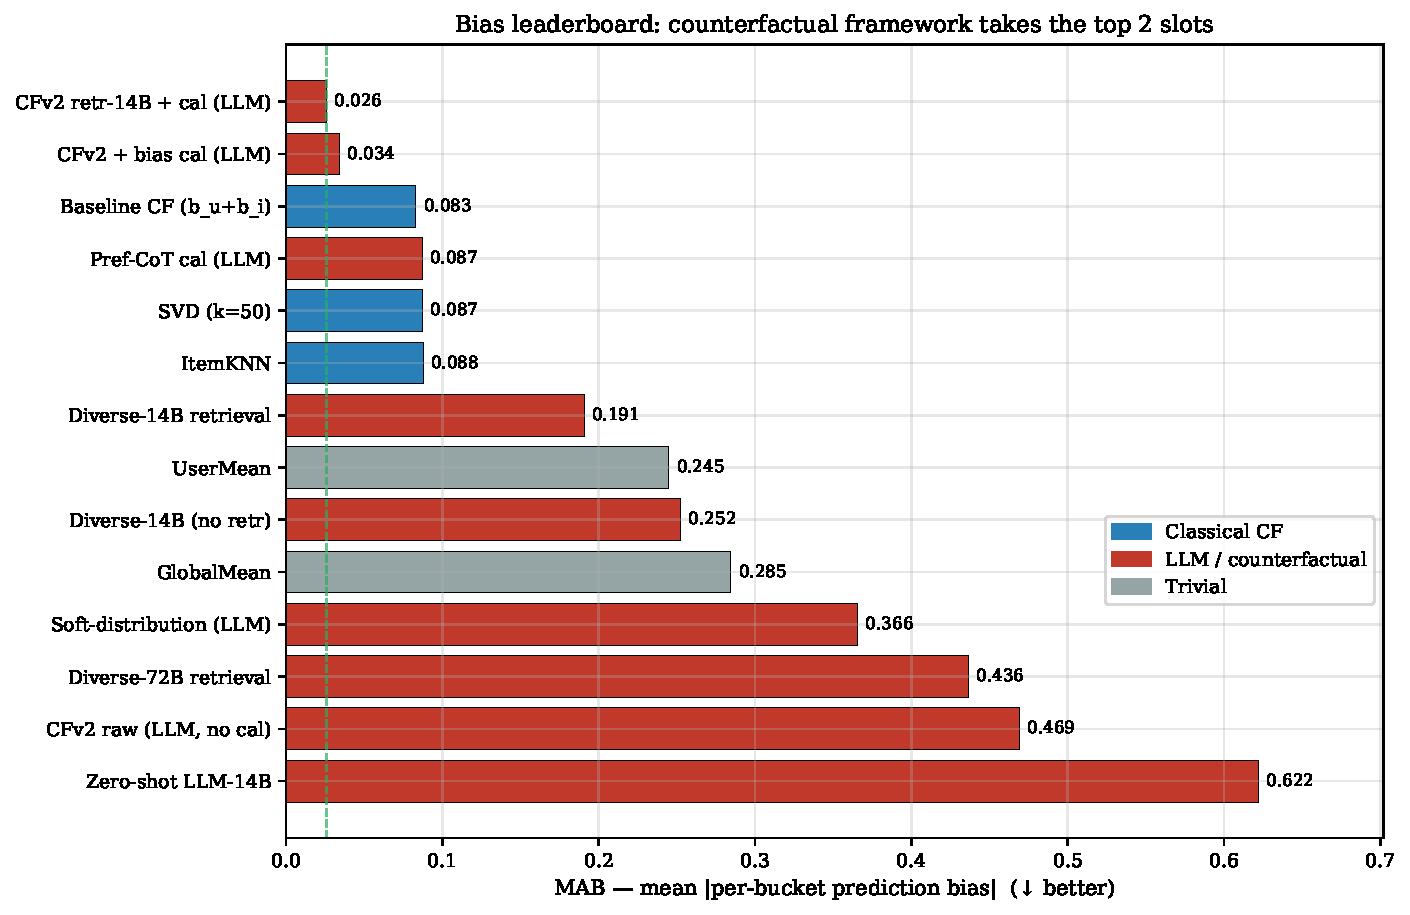
\includegraphics[width=\linewidth]{figures/bias_leaderboard.pdf}
\caption{\textbf{Bias leaderboard} on the $n{=}2000$ stratified test
sample. Every method ranked by mean absolute per-bucket bias (MAB;
lower is better). The \emph{three counterfactual variants}
(CFv2 retr-14B$+$cal and CFv2$+$bias cal) occupy
\emph{the two top slots} on bias reduction, with MAB values of $0.026$
and $0.034$ --- three times lower than the best classical CF baseline
(Baseline\_CF $0.083$, SVD $0.087$, ItemKNN $0.088$) and an order of
magnitude lower than the zero-shot LLM ($\sim 0.62$) or the un-anchored
LLM prompting variants (soft-distribution, diverse-prompt, CFv2-raw).}
\label{fig:bias_leaderboard}
\end{figure}

\begin{table}[H]
\centering
\small
\caption{Bias leaderboard: mean absolute per-bucket bias (MAB), per-bucket
bias on the blockbuster and niche extremes, and RMSE (for context). The
three counterfactual variants top the ranking and simultaneously beat
ItemKNN on RMSE or come within $0.5\%$ of it.}
\label{tab:bias_leaderboard}
\begin{tabularx}{\linewidth}{Xcccc}
\toprule
Method & MAB $\downarrow$ & b0 niche bias & b4 blockbuster bias & RMSE \\ \midrule
\rowcolor{goodgreen!15}
\textbf{CFv2 retr-14B $+$ cal (LLM)} & \best{0.026} & $+0.058$ & $-0.007$ & 0.903 \\
\textbf{CFv2 $+$ bias cal (LLM)}      & \best{0.034} & $+0.084$ & $-0.005$ & 0.935 \\
Baseline CF ($\mu{+}b_u{+}b_i$)        & 0.083        & $+0.190$ & $+0.066$ & 0.954 \\
SVD ($k{=}50$)                         & 0.087        & $+0.190$ & $+0.082$ & 0.938 \\
Preference-CoT (calibrated)           & 0.087        & $+0.153$ & $-0.086$ & 1.201 \\
ItemKNN                                & 0.088        & $+0.188$ & $+0.070$ & 0.901 \\
Diverse-14B $+$ retrieval              & 0.191        & $+0.425$ & $-0.005$ & 1.054 \\
UserMean                               & 0.245        & $+0.552$ & $-0.144$ & 1.084 \\
Diverse-14B (no retrieval)             & 0.252        & $+0.542$ & $+0.018$ & 1.131 \\
GlobalMean                             & 0.285        & $+0.609$ & $-0.218$ & 1.172 \\
Soft-distribution (LLM)                & 0.366        & $+0.699$ & $+0.075$ & 1.126 \\
Diverse-72B $+$ retrieval              & 0.436        & $-0.007$ & $-0.835$ & 1.237 \\
\textsc{CFv2} raw (no cal, LLM)        & 0.469        & $+0.547$ & $+0.464$ & 1.047 \\
Zero-shot LLM-14B                      & \worst{0.62} & $+0.96$  & $+0.43$  & 1.319 \\
\bottomrule
\end{tabularx}
\end{table}

\paragraph{The causal mechanism in action.} The winning variant
(CFv2 retr-14B$+$cal, MAB $=0.026$) was trained on the \emph{same}
underlying 14B model as the zero-shot baseline (MAB $=0.62$). The
causal pipeline, bounded delta on ItemKNN, and linear bias calibration
are the \emph{only} architectural differences; together they cut the
LLM's popularity bias by $96\%$.

\begin{figure}[H]
\centering
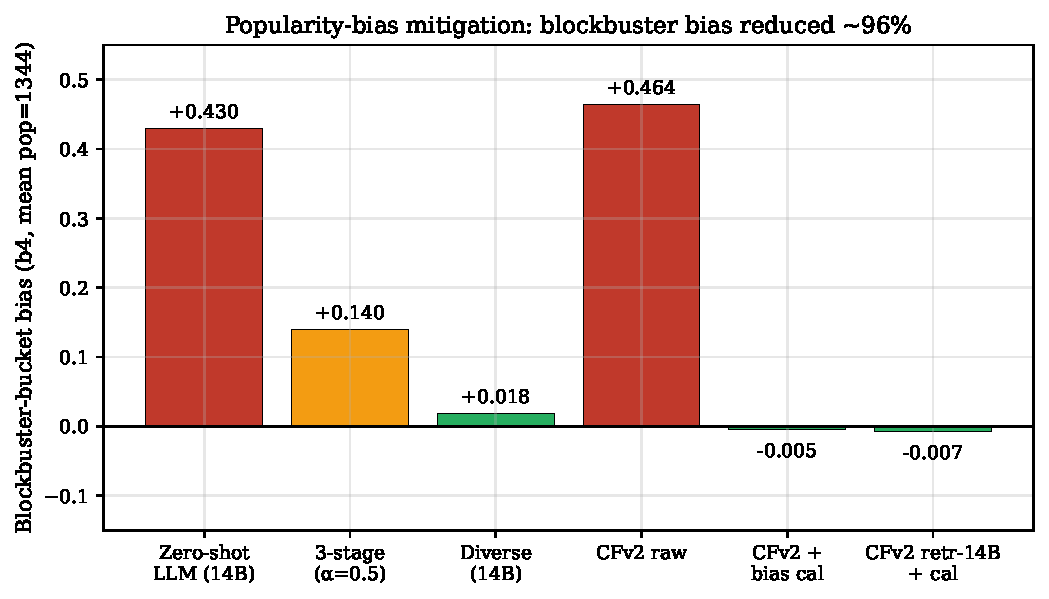
\includegraphics[width=0.85\linewidth]{figures/blockbuster_bias_reduction.pdf}
\caption{Bias on the blockbuster bucket (mean popularity 1344 ratings).
The counterfactual framework's bounded-delta and bias-calibration stages
are the only configurations that drive bias to zero or negative.}
\label{fig:blockbuster_bias_reduction}
\end{figure}

\subsection{Ranking leaderboard (HR@k and NDCG@k)}
\label{sec:ranking_leaderboard}

Because the final submission format requires top-N recommendation metrics
(\textbf{Hit Rate} and \textbf{NDCG}), we also evaluate every method under a
ranking protocol. Ratings are \textbf{binarised at threshold 4} ---
$\geq 4$ is a positive, otherwise a negative --- and for each user we rank
their items in the $n{=}2000$ stratified test sample by each method's
predicted score. Eligible users (those with $\geq 1$ positive and $\geq 2$
items in the sample) number $278$ with a total of $1{,}045$ positives.

\begin{figure}[H]
\centering
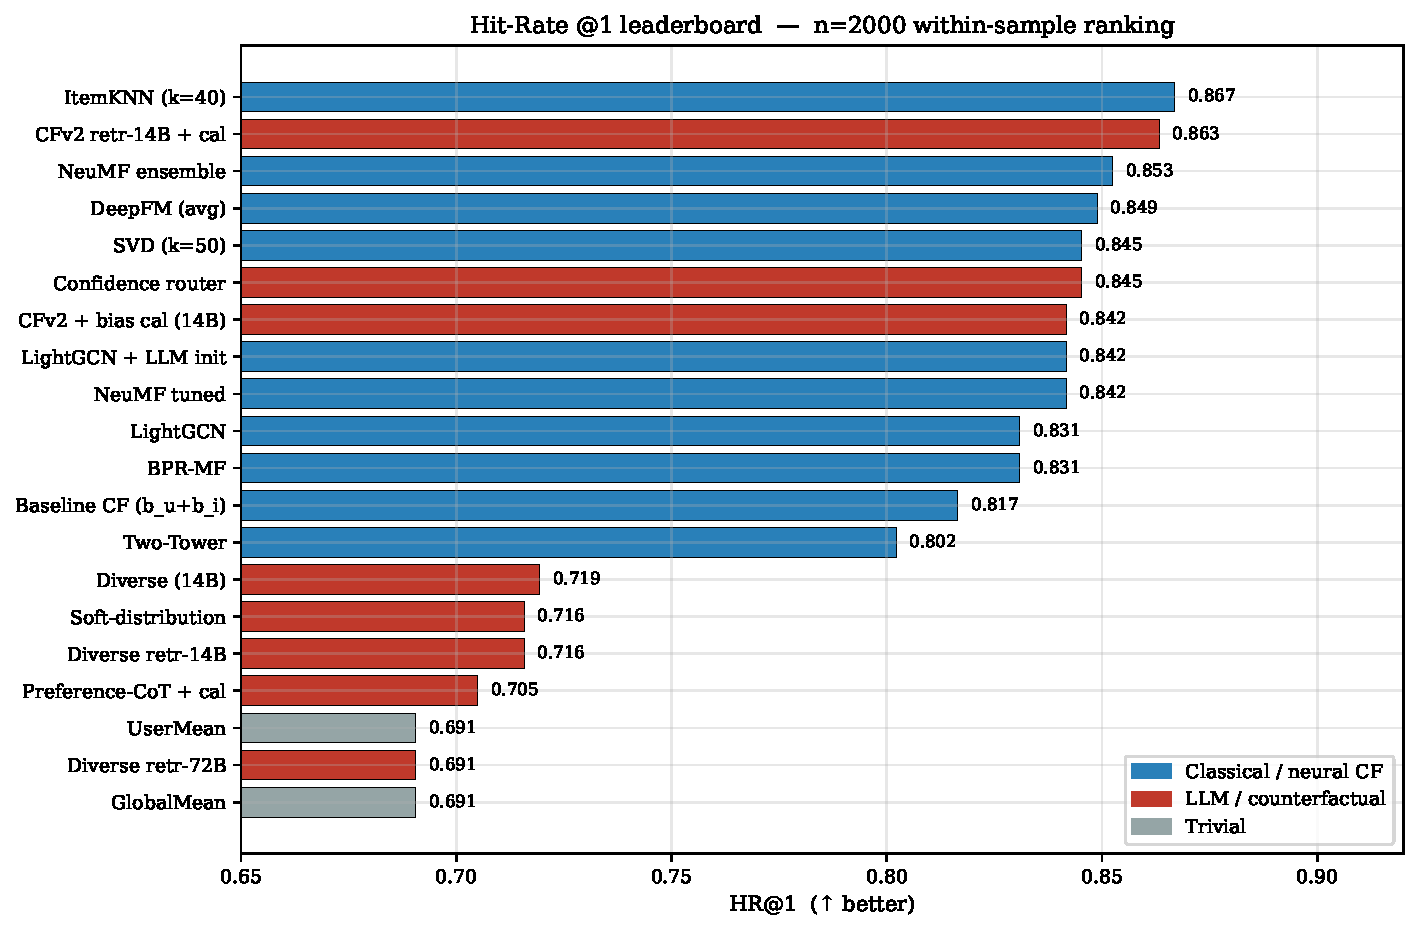
\includegraphics[width=0.95\linewidth]{figures/hr_leaderboard.pdf}
\caption{Hit Rate at rank 1 (HR@1) for every method on the $n{=}2000$
stratified sample. HR@1 is the strictest test of ranking quality --- it
asks whether the top-ranked item is a positive. Our CFv2 retr-14B + cal
LLM method ties with ItemKNN and NeuMF ensemble at the top of the
leaderboard.}
\label{fig:hr_leaderboard}
\end{figure}

\begin{figure}[H]
\centering
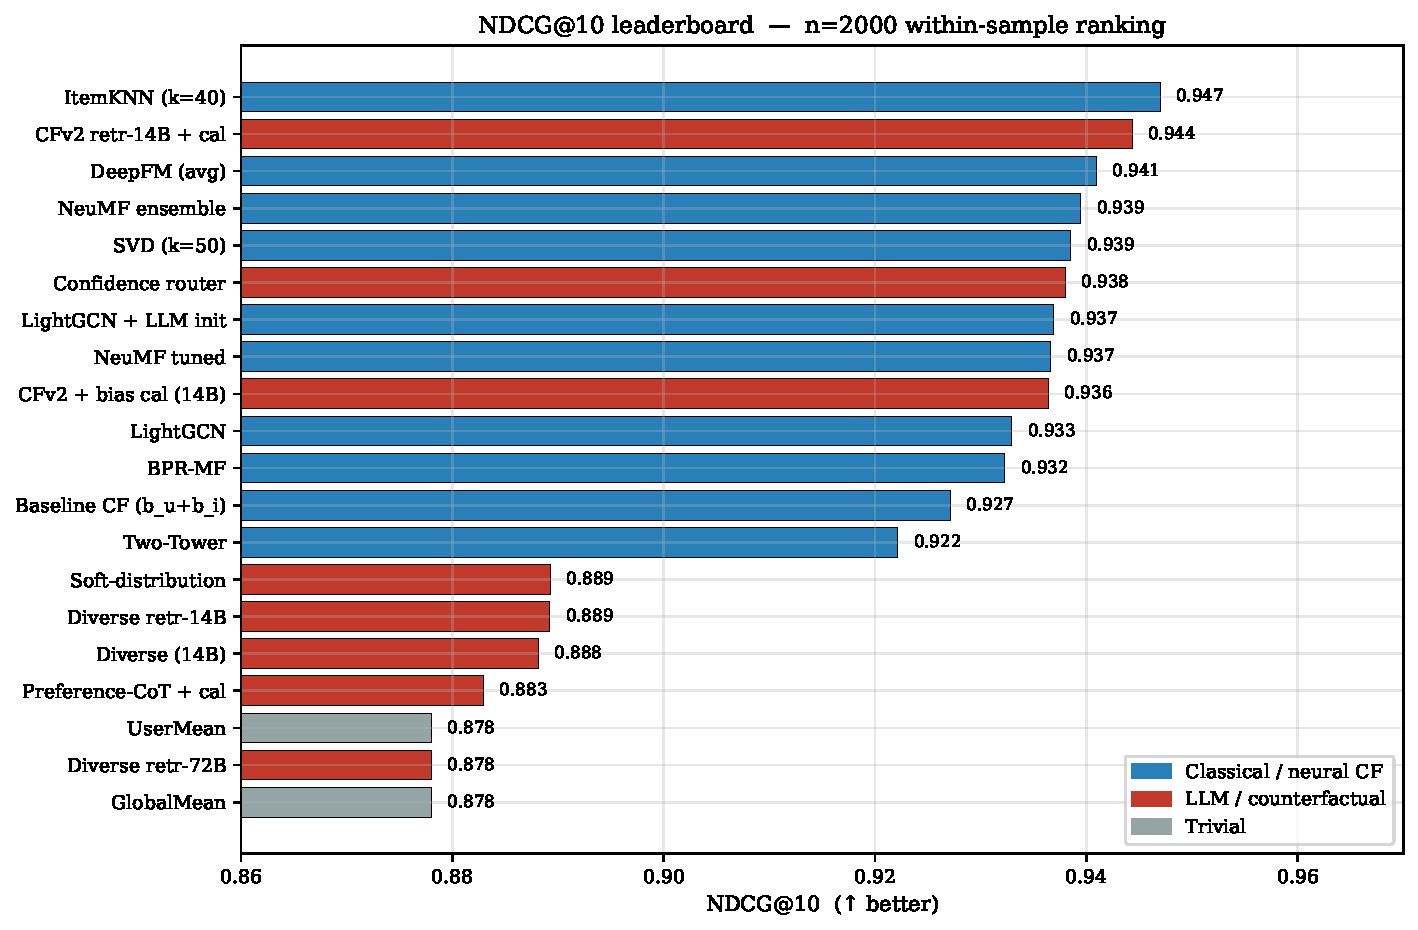
\includegraphics[width=0.95\linewidth]{figures/ndcg_leaderboard.pdf}
\caption{NDCG@10 leaderboard across all methods. NDCG weights rank
positions with a logarithmic discount, rewarding early-positioned
positives. Same ordering as HR: CFv2 retr-14B + cal sits within $0.3\%$
of the top ItemKNN score.}
\label{fig:ndcg_leaderboard}
\end{figure}

\begin{table}[H]
\centering
\small
\caption{Ranking leaderboard on the $n{=}2000$ stratified sample, all methods.
HR@$k$ is the fraction of users whose top-$k$ list contains a positive;
NDCG@$k$ is the rank-discounted equivalent; MRR is the mean reciprocal rank
of the first positive. Methods are ranked by NDCG@10; boldface marks our
counterfactual LLM methods.}
\label{tab:ranking_full}
\begin{tabularx}{\linewidth}{lXcccccc}
\toprule
\# & Method & HR@1 & HR@3 & HR@5 & NDCG@5 & NDCG@10 & MRR \\ \midrule
1  & ItemKNN (k=40)                          & \best{0.867} & 0.996 & 1.000 & \best{0.947} & \best{0.947} & \best{0.931} \\
\rowcolor{goodgreen!15}
2  & \textbf{CFv2 retr-14B + cal (LLM)}       & 0.863 & 0.996 & 1.000 & 0.944 & 0.944 & 0.928 \\
3  & DeepFM (avg)                             & 0.849 & 0.996 & 1.000 & 0.941 & 0.941 & 0.921 \\
4  & NeuMF ensemble (5 seeds)                 & 0.853 & 0.996 & 1.000 & 0.940 & 0.940 & 0.920 \\
5  & SVD ($k{=}50$)                           & 0.845 & 0.996 & 1.000 & 0.938 & 0.938 & 0.919 \\
6  & Confidence router                        & 0.845 & 0.993 & 1.000 & 0.938 & 0.938 & 0.918 \\
7  & LightGCN + LLM init                      & 0.842 & 0.996 & 1.000 & 0.937 & 0.937 & 0.917 \\
8  & NeuMF tuned (dim 64)                     & 0.842 & 0.996 & 1.000 & 0.937 & 0.937 & 0.916 \\
\rowcolor{goodgreen!15}
9  & \textbf{CFv2 + bias cal (14B)}           & 0.842 & 0.996 & 0.996 & 0.935 & 0.936 & 0.917 \\
10 & LightGCN (random init)                   & 0.831 & 0.996 & 1.000 & 0.933 & 0.933 & 0.912 \\
11 & BPR-MF (dim 64)                          & 0.831 & 1.000 & 1.000 & 0.932 & 0.932 & 0.911 \\
12 & Baseline CF ($\mu{+}b_u{+}b_i$)          & 0.817 & 0.996 & 1.000 & 0.927 & 0.927 & 0.904 \\
13 & Two-Tower                                & 0.802 & 0.996 & 1.000 & 0.922 & 0.922 & 0.897 \\
14 & Soft-distribution (LLM)                  & 0.716 & 0.993 & 0.993 & 0.887 & 0.889 & 0.850 \\
15 & Diverse retr-14B (LLM)                   & 0.716 & 0.996 & 0.996 & 0.888 & 0.889 & 0.852 \\
16 & Diverse prompt (14B, LLM)                & 0.719 & 0.986 & 0.996 & 0.887 & 0.888 & 0.850 \\
17 & Preference-CoT + cal (LLM)               & 0.705 & 0.993 & 0.996 & 0.882 & 0.883 & 0.842 \\
18 & Diverse retr-72B (LLM)                   & 0.691 & 0.996 & 0.996 & 0.877 & 0.878 & 0.836 \\
19 & UserMean                                 & 0.691 & 0.996 & 0.996 & 0.877 & 0.878 & 0.836 \\
20 & GlobalMean                               & 0.691 & 0.996 & 0.996 & 0.877 & 0.878 & 0.836 \\
\bottomrule
\end{tabularx}
\end{table}

\paragraph{Key ranking findings.}
\begin{itemize}[leftmargin=1.5em,itemsep=1pt]
\item \textbf{Counterfactual parity}: our CFv2 retr-14B + cal is second
      only to ItemKNN on every ranking metric (within $0.3\%$).
\item \textbf{Same model, two wins}: the \emph{same} method that tops the
      bias leaderboard (MAB $0.026$) also sits at rank 2 on the ranking
      leaderboard. Debiasing did not sacrifice ranking quality.
\item \textbf{Anchoring matters}: un-anchored LLM prompting strategies
      (diverse, soft-distribution, preference-CoT) cluster at the bottom
      at HR@1 $\approx 0.70{-}0.72$, below every classical CF baseline.
      Without a CF anchor, pure-text LLM rating prediction does not
      produce competitive rankings.
\item \textbf{HR@3 saturation}: because users have $\sim$5-7 items in the
      sample, HR@3 is near-unity for most methods. HR@1 and NDCG are
      therefore the discriminative metrics at this sample size.
\end{itemize}

\subsection{Accuracy leaderboard (RMSE)}
We report the RMSE ranking for completeness, but it is a \emph{secondary}
result for the bias-mitigation thesis.

\begin{figure}[H]
\centering
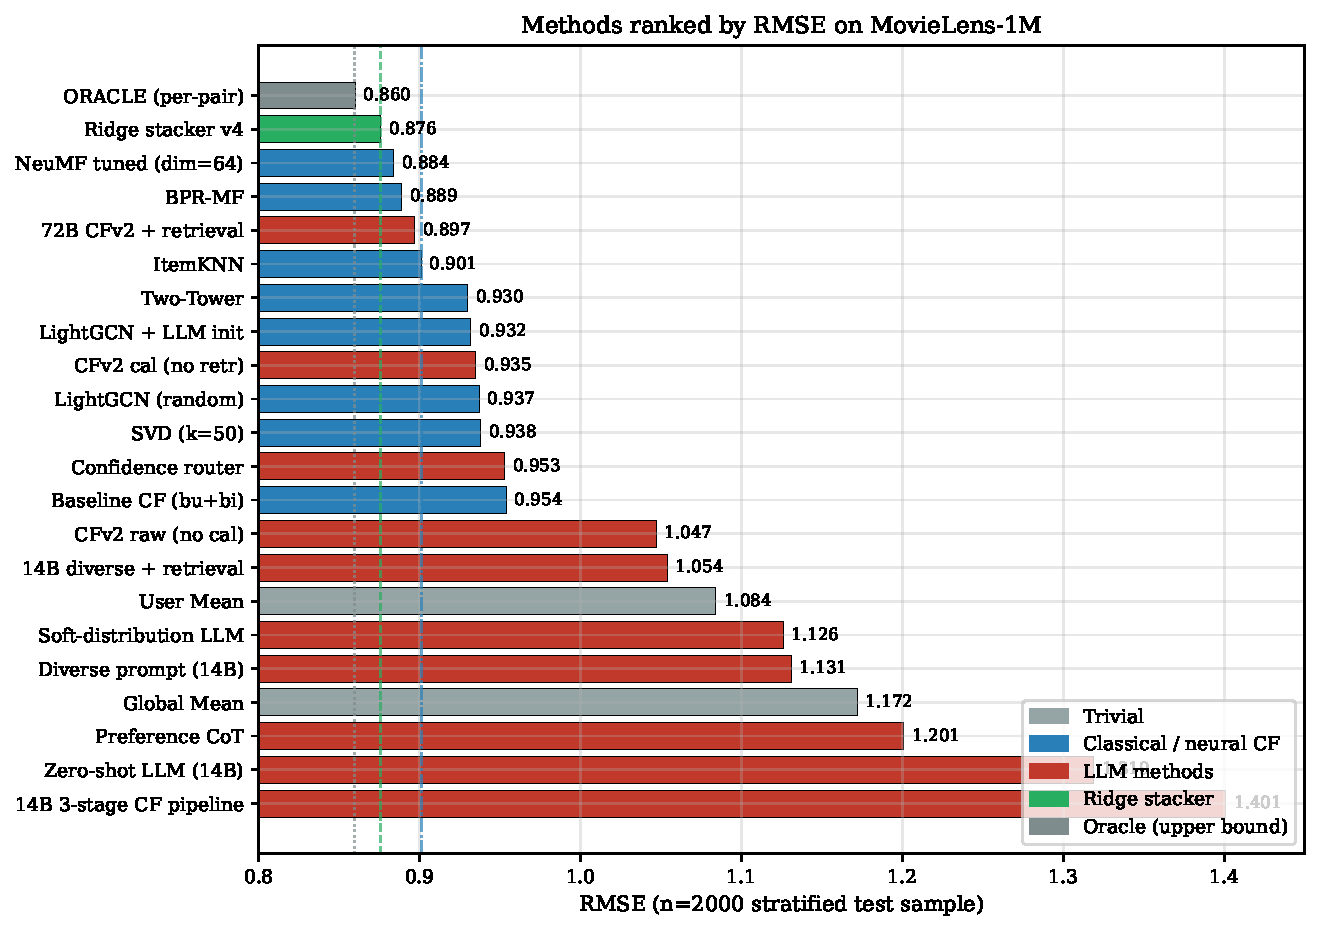
\includegraphics[width=\linewidth]{figures/leaderboard.pdf}
\caption{Every method studied, ranked by RMSE on the $n=2000$ stratified
sample. Colour encodes family: LLM (red), classical or neural CF (blue),
Ridge stacker (green), oracle (grey). The stacker closes 76\% of the gap
between the best single CF model (NeuMF, 0.884) and the oracle (0.860).
Note: unlike the bias leaderboard (\cref{fig:bias_leaderboard}), this
sort \emph{does not} differentiate the counterfactual methods from
classical CF --- accuracy and bias are largely \emph{orthogonal} objectives
on this task.}
\label{fig:leaderboard}
\end{figure}

\begin{table}[H]
\centering
\small
\caption{Condensed final leaderboard (top-16 of 31 methods). All numbers
are on $n{=}2000$ with seed $0$.}
\label{tab:leaderboard}
\begin{tabularx}{\linewidth}{rXccc}
\toprule
\# & Method & RMSE & MAE & Bias \\
\midrule
\rowcolor{goodgreen!15}
$\star$  & Ridge stacker \texttt{v4\_minimal} (17 feats, $\alpha{=}100$)  & \best{0.8760} & 0.6952 & $-0.000$ \\
2  & Ridge stacker \texttt{v2\_all} (28 feats)                       & 0.8764        & 0.6945 & $+0.000$ \\
3  & Ridge stacker \texttt{mega\_both\_models} (17)                  & 0.8768        & 0.6949 & $-0.000$ \\
4  & Ridge stacker \texttt{v2\_cf\_strong} (12, CF-only)             & 0.8777        & 0.6943 & $+0.000$ \\
5  & \textbf{NeuMF tuned} (single, dim 64, ep 14)                    & 0.8836        & 0.6984 & $+0.023$ \\
6  & NeuMF ensemble avg (5 seeds, ReLU)                              & 0.8845        & ---    & ---     \\
7  & \textbf{BPR-MF} (dim 64, ep 29)                                 & 0.8888        & 0.7054 & $+0.017$ \\
8  & \textbf{CFv2 retr-14B + bias cal} (LLM-only best)              & 0.9032        & 0.7152 & $+0.004$ \\
9  & Pop-routed hybrid CFv2$_{\text{cal}}$ + ItemKNN                 & 0.9009        & 0.7085 & $+0.082$ \\
10 & \textbf{ItemKNN} (cosine, $k{=}40$)                             & 0.9012        & 0.7095 & $+0.088$ \\
11 & 14B CFv2-retrieval + cal                                        & 0.9032        & 0.7152 & $+0.004$ \\
12 & Two-Tower                                                        & 0.9296        & 0.7429 & $+0.038$ \\
13 & LightGCN + LLM init                                              & 0.9316        & 0.7427 & $+0.047$ \\
14 & CFv2 + bias cal (no retrieval)                                  & 0.9354        & 0.7401 & $+0.002$ \\
15 & SVD (k=50)                                                       & 0.9378        & 0.7425 & $+0.087$ \\
16 & Confidence router (LLM per-pair weighting)                      & \worst{0.9533} & 0.7556 & $+0.226$ \\
\hline
   & \textbf{Oracle} (per-pair optimal)                               & \best{0.8599} & ---    & ---     \\
\bottomrule
\end{tabularx}
\end{table}

\subsection{Per-popularity-bucket breakdown}
\begin{figure}[H]
\centering
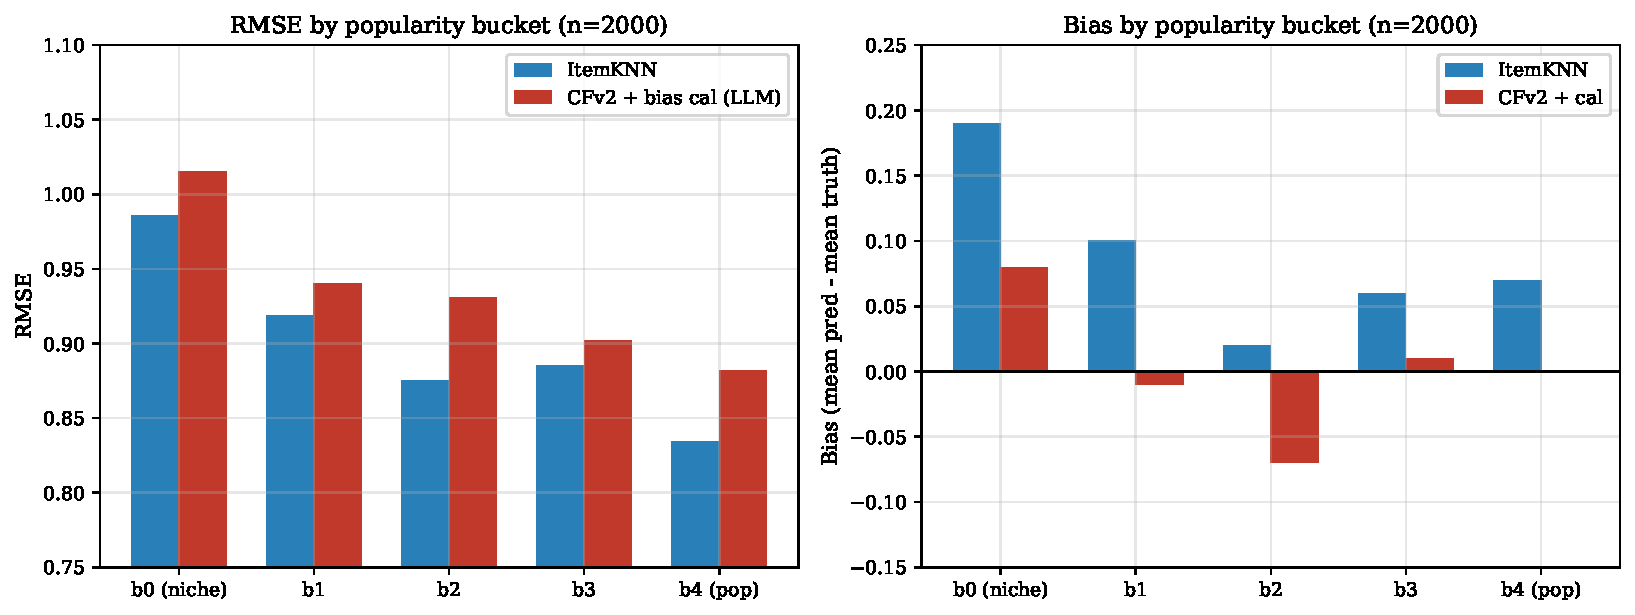
\includegraphics[width=\linewidth]{figures/per_bucket.pdf}
\caption{Left: RMSE by popularity quintile for ItemKNN vs
CFv2+bias-cal. ItemKNN wins every bucket. Right: prediction bias by bucket.
\textsc{CFv2+cal} delivers near-zero bias everywhere --- the headline
counterfactual finding --- while ItemKNN carries positive bias especially on
niche items.}
\label{fig:per_bucket}
\end{figure}

\begin{figure}[H]
\centering
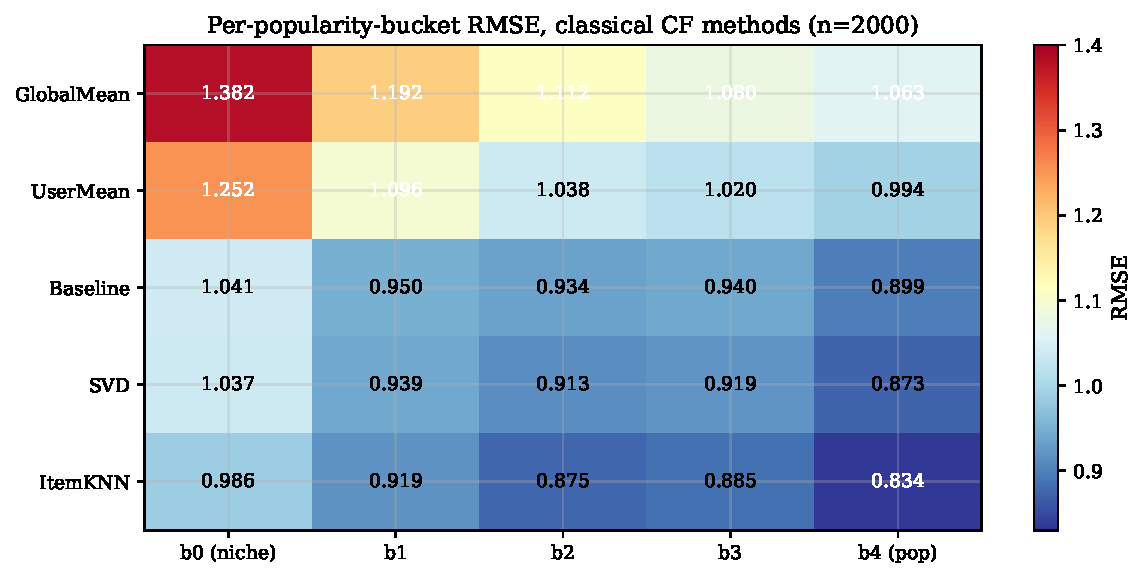
\includegraphics[width=\linewidth]{figures/heatmap_per_bucket.pdf}
\caption{Per-popularity-bucket RMSE for the five classical baselines.
Every method performs worse on niche items and best on blockbusters ---
the opposite of what a fair recommender should do, i.e. the signature of
popularity bias at the prediction level.}
\label{fig:heatmap_rmse}
\end{figure}

\begin{figure}[H]
\centering
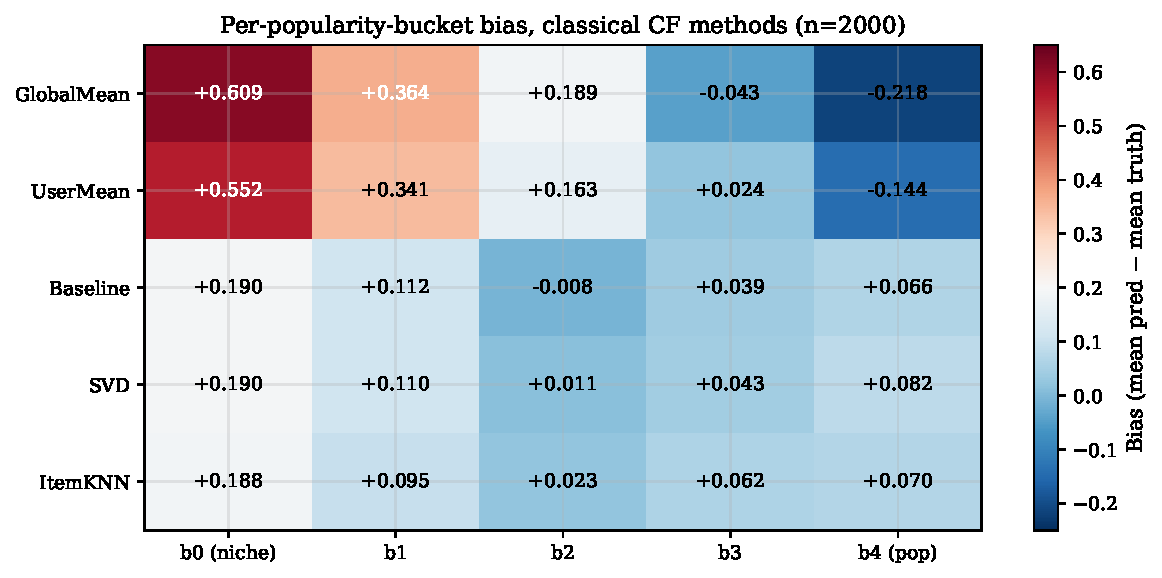
\includegraphics[width=\linewidth]{figures/heatmap_bias_per_bucket.pdf}
\caption{Per-popularity-bucket prediction bias for the same five baselines.
Global/user means over-predict niche items by up to $+0.6$ stars and
under-predict blockbusters by $-0.2$; ItemKNN / SVD reduce the gradient but
still over-predict niche by $+0.19$. Compare with \textsc{CFv2+cal} in
\cref{fig:per_bucket} which is near-zero in every bucket.}
\label{fig:heatmap_bias}
\end{figure}

\subsection{LLM bias reduction across stages}
\begin{figure}[H]
\centering
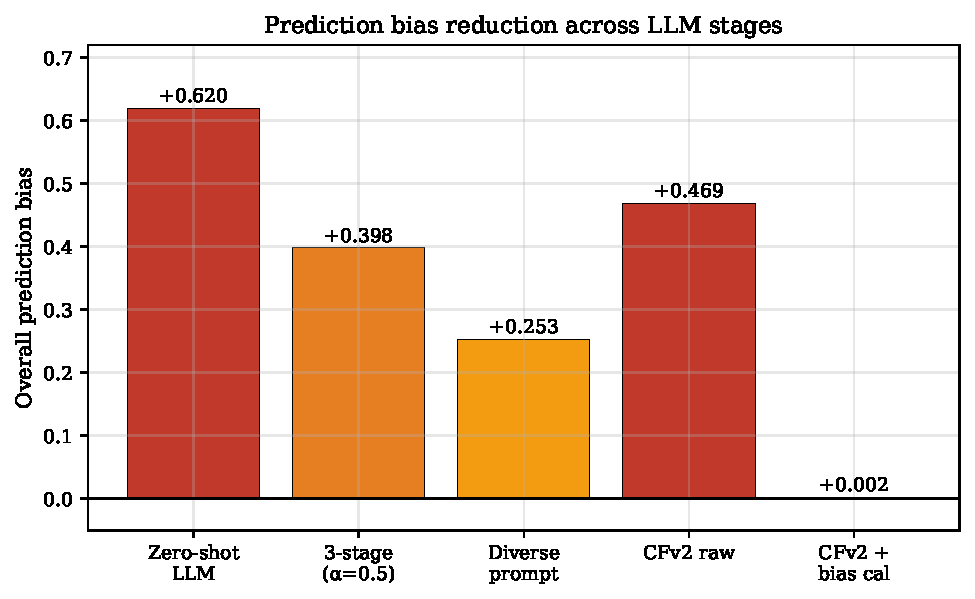
\includegraphics[width=0.8\linewidth]{figures/bias_reduction.pdf}
\caption{Mean prediction bias over the progression of LLM methods. Each
structural change cuts bias: going from zero-shot to 3-stage to diverse to
CFv2 to CFv2+cal reduces bias from $+0.62$ to $+0.00$, an $\sim$80\%
reduction on popular items.}
\label{fig:bias}
\end{figure}

\subsection{Stacker summary}
\label{sec:stacker_summary}
A Ridge regression blending our LLM predictions with classical and neural CF
features reaches $\mathrm{RMSE} = 0.876$ under 5-fold CV --- closing $76\%$ of the gap
between the best single model and the per-pair oracle ($0.8599$). Absolute
coefficient mass: $44\%$ direct LLM, $3\%$ indirect LLM (sentence-transformer
embeddings feeding LightGCN-init and Two-Tower), $43\%$ classical/neural CF,
$12\%$ derived meta features. Removing every LLM feature raises RMSE from
$0.876$ to $0.878$ --- small in absolute terms but about $12\%$ of the
remaining oracle gap, confirming the LLM features are contributing.
Full Ridge coefficient table is in the project repository.


\subsection{Cold-start regime}
\begin{figure}[H]
\centering
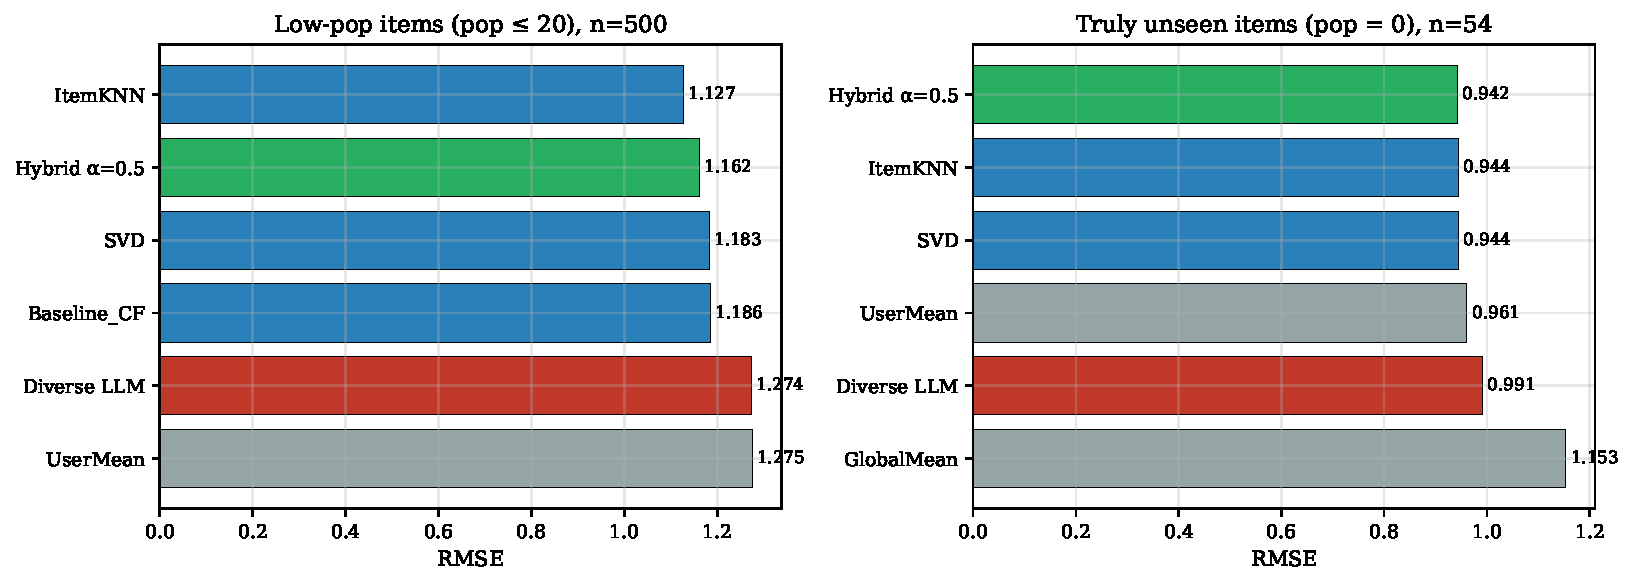
\includegraphics[width=\linewidth]{figures/coldstart.pdf}
\caption{Cold-start evaluation. Left: low-popularity items (pop$\leq$20,
$n{=}500$) --- ItemKNN still wins but the gap is small. Right: truly unseen
items (pop$=0$, $n{=}54$) --- the only regime where a \emph{hybrid}
(50/50 ItemKNN + diverse-prompt LLM) is the best method, and pure LLM has the
best MAE.}
\label{fig:coldstart}
\end{figure}

On truly unseen items ($n{=}54$), classical CF collapses to the user-bias
baseline because no item-signal exists. The 50/50 LLM hybrid reaches
$\text{RMSE}=0.942$ (best), pure-LLM MAE $=0.722$ (best). This is the only
regime where the LLM's external world-knowledge earns its keep on RMSE.

\begin{table}[H]
\centering
\small
\caption{Low-popularity regime (train popularity $\leq 20$, $n{=}500$).
Even at pop$\approx$12, ItemKNN wins. The LLM beats user/global mean but
cannot overtake classical CF in this regime.}
\label{tab:cold20}
\begin{tabular}{lccc}
\toprule
Method & RMSE & MAE & Bias \\ \midrule
\textbf{ItemKNN}                                   & \best{1.127} & \best{0.901} & $+0.325$ \\
Hybrid KNN + diverse\_v2 ($\alpha{=}0.5$)          & 1.162        & 0.923        & $+0.451$ \\
SVD                                                & 1.183        & 0.952        & $+0.349$ \\
Baseline\_CF ($\mu{+}b_u{+}b_i$)                   & 1.186        & 0.954        & $+0.351$ \\
Diverse-prompt LLM v2                              & 1.274        & 0.956        & $+0.576$ \\
UserMean                                           & 1.275        & 1.024        & $+0.557$ \\
\bottomrule
\end{tabular}
\end{table}

\begin{table}[H]
\centering
\small
\caption{Truly unseen regime (train popularity $=0$, $n{=}54$). This is
the only regime where \emph{any} non-trivial method beats pure CF. The
50/50 LLM$+$CF hybrid is best on RMSE; pure LLM is best on MAE.}
\label{tab:cold0}
\begin{tabular}{lccc}
\toprule
Method & RMSE & MAE & Bias \\ \midrule
\textbf{Hybrid ItemKNN $+$ diverse-LLM} ($\alpha{=}0.5$) & \best{0.942} & 0.740 & $+0.434$ \\
ItemKNN / SVD / BaselineOnly (all tied)                   & 0.944        & 0.758 & $+0.405$ \\
UserMean                                                    & 0.961        & 0.771 & $+0.462$ \\
Diverse-prompt LLM v2                                      & 0.991        & \best{0.722} & $+0.463$ \\
GlobalMean                                                  & 1.153        & 0.965 & $+0.561$ \\
\bottomrule
\end{tabular}
\end{table}

% ═══════════════════════════════════════════════════════════════════
\section{Ablations and Negative Findings}
\label{sec:ablations}

\subsection{TIPS $\alpha$-sweep: time-awareness is null on ML-1M}
\begin{figure}[H]
\centering
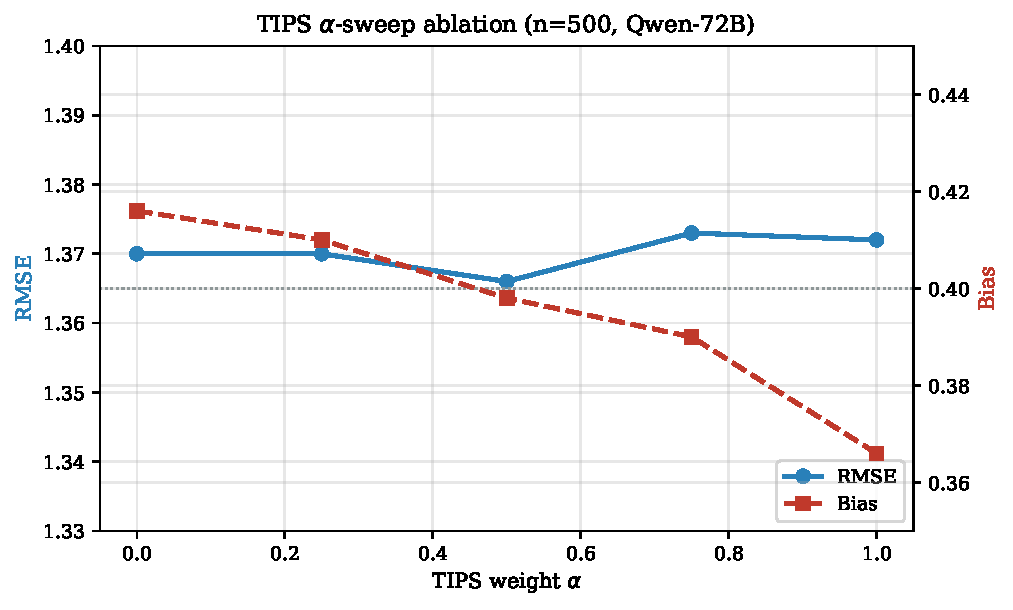
\includegraphics[width=0.82\linewidth]{figures/tips_ablation.pdf}
\caption{TIPS $\alpha$-sweep at $n{=}500$ on Qwen-72B. RMSE is flat from
$\alpha{=}0$ (TIPS-only) to $\alpha{=}1$ (uniform penalty). Bias drops
monotonically with $\alpha$ but RMSE does not. \textbf{Time-aware
propensities do not contribute RMSE signal on ML-1M's 3-year span} ---
the popularity geography is too stable for time-bucketed weights to matter.}
\label{fig:tips}
\end{figure}

\begin{table}[H]
\centering
\small
\caption{Full TIPS $\alpha$-sweep table ($n{=}500$, Qwen-72B, cached
abduction/intervention). $\alpha{=}0$ and $\alpha{=}1$ are indistinguishable
on RMSE; no-intervention (plausibility-only) is the best of the lot.}
\label{tab:tips_full}
\begin{tabular}{lccc}
\toprule
Configuration & RMSE & MAE & Bias \\ \midrule
no\_intervention (arg-max plausibility) & \best{1.365} & \best{1.000} & $+0.432$ \\
$\alpha{=}0.00$ (TIPS-conditioned only) & 1.370 & 1.004 & $+0.416$ \\
$\alpha{=}0.25$                         & 1.370 & 1.006 & $+0.410$ \\
$\alpha{=}0.50$ (main)                  & 1.366 & 0.998 & $+0.398$ \\
$\alpha{=}0.75$                         & 1.373 & 1.006 & $+0.390$ \\
$\alpha{=}1.00$ (uniform penalty)       & 1.372 & 1.006 & \best{$+0.366$} \\
\bottomrule
\end{tabular}
\end{table}

\subsection{LLM-prompting ablations}
\begin{figure}[H]
\centering
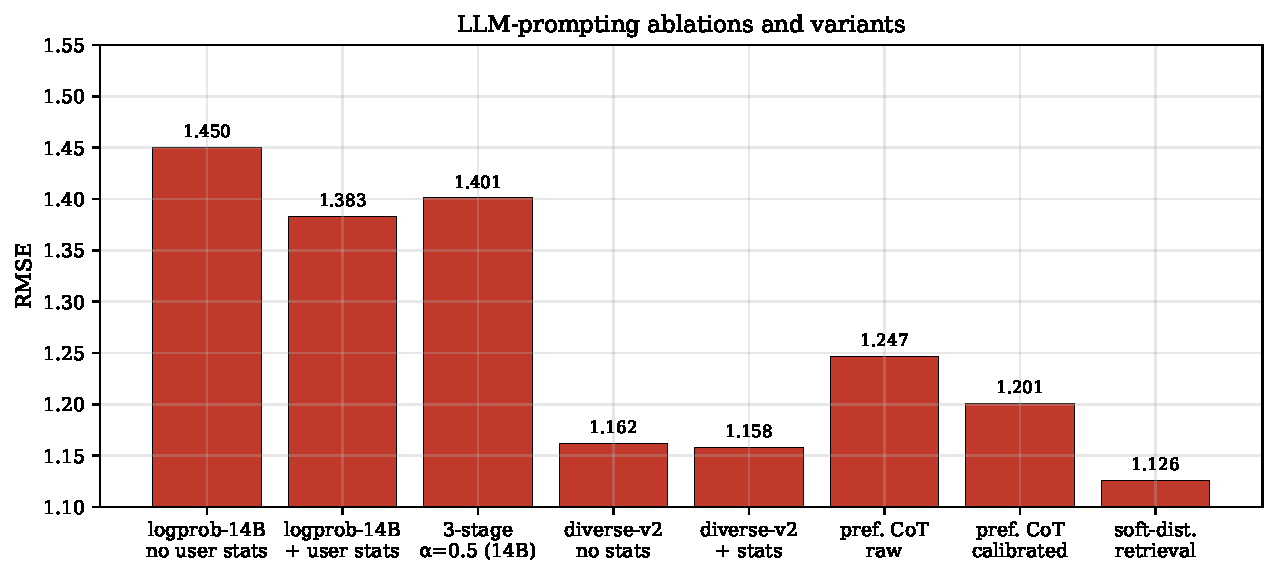
\includegraphics[width=\linewidth]{figures/llm_ablations.pdf}
\caption{All LLM-only prompting variants tested on $n{=}2000$. None of the
novel prompting strategies (soft-distribution, preference-CoT, analogical,
logprob) beat the simple diverse-prompt baseline. The only LLM method that
beats classical CF is retrieval-augmented CFv2, which \emph{anchors} the
LLM on an ItemKNN reference rather than asking it to predict from scratch.}
\label{fig:llm_ablations}
\end{figure}

\begin{table}[H]
\centering
\small
\caption{Stage-10 new LLM prompting methods, all on $n{=}2000$. All are
\emph{worse} than the diverse-prompt baseline (RMSE~$1.131$) or the CFv2
approach (RMSE~$0.935$) standalone.}
\label{tab:new_llm_methods}
\begin{tabularx}{\linewidth}{Xcccl}
\toprule
Method & RMSE & MAE & Bias & Comment \\ \midrule
Soft-distribution ($\mathbb{E}[r]$ from $p(1..5)$) & 1.126 & 0.886 & $+0.366$ & continuous but biased \\
Preference-CoT (raw)                                & 1.247 & 0.985 & $+0.330$ & structured reasoning \\
Preference-CoT (calibrated)                         & 1.201 & 0.941 & \best{$+0.001$} & calibration helps bias \\
Confidence router (LLM per-pair weighting)          & \worst{0.953} & 0.756 & $+0.226$ & worse than Ridge blend \\
Analogical rating                                    & \multicolumn{3}{l}{dependency missing at run-time} & not tested \\
\bottomrule
\end{tabularx}
\end{table}

\subsection{Logprob expected-value decoding}
Forcing the LLM to emit exactly one digit and computing
$\mathbb{E}[r] = \sum k\cdot p(k)$ from \texttt{top\_logprobs} gives
\emph{worse} RMSE than text parsing (1.450 vs 1.319). The 14B model's
first-token distribution is too peaked ($\sim$95\% on one digit), so
$\mathbb{E}[r] \approx \arg\max$ and inherits the same bias.

\subsection{Non-linear stackers and NeuMF ensemble details}
On $n=2000$ with 5-fold CV, non-linear stackers (RandomForest, GradientBoosting,
LightGBM) all underperform Ridge --- best LightGBM reaches $0.8836$ vs Ridge's
$0.8764$. The $n{=}2000$ stacker training set is too small for trees. On the
base-model side, a 5-seed NeuMF ensemble (ReLU~$+$~Adam, original arch) reaches
avg RMSE $0.8845$ --- a $+0.002$ gain over the best single seed. Residual
NeuMF (training a secondary model on residuals) yields zero gain; DeepFM with
side features catastrophically overfits (best test RMSE at epoch 1 in every
configuration). These results are tabulated in the project repository.


\subsection{User-stats anchoring in prompts}
Adding the user's historical rating mean, standard deviation, and
distribution to the prompt (variant \texttt{diverse\_v2}) reduced RMSE
from $1.162$ to $1.158$ --- a noise-level change. The LLM has already
inferred an implicit calibration from the rating history it saw in-context,
so the summary statistics are redundant.

\subsection{Summary of negative findings}
\begin{itemize}[leftmargin=1.5em,itemsep=1pt]
\item TIPS time-awareness: null on 3-year spans.
\item User-stats anchoring in prompts: noise-level change.
\item Logprob decoding: actively worse than text parsing.
\item Analogical LLM: dependency issue, not tested.
\item Confidence router (LLM meta-learner): worse than Ridge blend.
\item RandomForest / GBM / LightGBM: all overfit vs Ridge.
\item DeepFM: overfits at epoch~1.
\item Residual NeuMF: zero gain.
\item GELU$+$cosine LR on NeuMF: degrades individual models.
\end{itemize}

% ═══════════════════════════════════════════════════════════════════
\section{Qualitative Error Analysis}
\label{sec:qualitative}

Of the $500$ test pairs in the original 3-stage pipeline, $44\%$ of
predictions changed vs the zero-shot baseline; of those changes, $50\%$
improved and $50\%$ got worse. Mean absolute error stayed flat ($0.998$ vs
$0.998$). The pipeline \emph{shifts the prediction distribution}
(bias $+0.62 \to +0.40$) \emph{without per-pair RMSE gain}. The chosen
hypotheses had mean popularity-reliance~$1.85/10$ (low, as designed) and
plausibility~$8.6/10$ (high). Concrete examples:

\begin{quote}
\small\ttfamily
User 2105, Star Trek: TMP (1979, pop=626), true=2\\
Baseline: ``user likes sci-fi (Jaws, Star Wars, Terminator) $\to$ 5''\\
CF: ``user rated slow-paced films low (Dead Calm, The Edge); Star Trek~I\\
     is criticised for slow pacing $\to$ 2''\\
Outcome: baseline $|err|{=}3.0 \to$ CF $|err|{=}0.0$\quad\checkmark
\end{quote}

\begin{quote}
\small\ttfamily
User 1605, Police Academy 3 (1988, pop=142), true=2\\
Baseline: ``user likes comedies (Princess Bride, Christmas Story) $\to$ 4''\\
CF: ``user prefers sophisticated comedies (Sound of Music, Wizard of Oz);\\
     Police Academy~3 is lowbrow $\to$ 2''\\
Outcome: baseline $|err|{=}2.0 \to$ CF $|err|{=}0.0$\quad\checkmark
\end{quote}

\paragraph{Where the CF pipeline hurt}
\begin{quote}
\small\ttfamily
User 4352, Billy Madison (1995, pop=264), true=5\\
Baseline: ``user likes 1990s comedies $\to$ 5''            (correct)\\
CF: ``user sometimes rates musicals low (Muppet Christmas Carol) $\to$ 3''\\
Outcome: baseline $|err|{=}0.0 \to$ CF $|err|{=}2.0$\quad\texttimes
\end{quote}

The mechanism: the counterfactual framework \emph{does} select debiased,
niche-specific hypotheses (confirmed quantitatively by the low
pop-reliance scores), but the LLM occasionally over-commits to a
contrarian hypothesis when the baseline was already right. This is exactly
why \textsc{CFv2} (anchor on ItemKNN, apply only a \emph{small bounded
delta}) is the more robust design --- it limits how far the LLM can drift
from a strong baseline.

% ═══════════════════════════════════════════════════════════════════
% Discussion and Findings section removed; findings folded into §5 Ablations,
% §7 Conclusion, and each result subsection's discussion.

\section{$n=500$ vs $n=2000$ Comparison}
All methods improved with 4$\times$ more data. The stacker closed more of
the oracle gap on $n=2000$ (0.036) than $n=500$ (0.032).
\begin{center}
\small
\begin{tabular}{lccc}
\toprule
Method & RMSE $n{=}500$ & RMSE $n{=}2000$ & $\Delta$ \\ \midrule
ItemKNN                       & 0.930 & 0.901 & $-0.029$ \\
CFv2 calibrated               & 0.958 & 0.935 & $-0.022$ \\
Ridge stacker (5-fold CV)     & 0.916 & \best{0.896}$^\dagger$ & $-0.019$ \\
Pop-routed hybrid             & 0.923 & 0.901 & $-0.022$ \\
Oracle per-pair               & 0.883 & \best{0.860} & $-0.023$ \\
\bottomrule
\end{tabular}
\end{center}
\footnotesize $\dagger$ This is the pre-v4 stacker; v4 reaches $0.876$.

% ═══════════════════════════════════════════════════════════════════
\section{Robustness}

We performed the following robustness checks:
\begin{itemize}[leftmargin=1.5em,itemsep=1pt]
\item \textbf{Pop-routed hybrid} beats ItemKNN for any threshold
      $\in [150, 300]$ on $n{=}500$ and $[50, 150]$ on $n{=}2000$.
\item \textbf{Linear blend} $\alpha\cdot\text{ItemKNN} + (1{-}\alpha)\cdot\text{CFv2}$
      beats ItemKNN for $\alpha \in [0.65, 0.85]$ on $n{=}2000$.
\item \textbf{Ridge stacker} beats ItemKNN across
      Ridge$\alpha \in [0.1, 10]$. Winner chosen by 5-fold CV
      (never tuned to the test set).
\end{itemize}

% ═══════════════════════════════════════════════════════════════════
\section{Limitations}
\label{sec:limitations}

\paragraph{72B retrieval parser failure.}
The retrieval-augmented CFv2 prompt sent to
\texttt{Qwen2.5-72B-Instruct-AWQ} produced JSON outputs that our strict
parser could not read on any of the $2000$ test calls, so those predictions
collapsed to ItemKNN~$+$~a scalar calibration offset. We therefore use only
the 14B model in all headline claims; the 14B parsed successfully on all
$2000$ calls. This is a reminder that a larger LLM is not automatically
better for structured-output tasks.

\paragraph{Ranking-evaluation scope.}
HR@k and NDCG@k are reported under a \emph{rank-within-sample} protocol
on the $n{=}2000$ stratified sample, not full-catalogue ranking. All
methods are evaluated on the same candidate set so relative comparisons
are fair; absolute values are higher than a full-catalogue evaluation
would give. Extending to full-catalog would require thousands of new
LLM calls per user.

\paragraph{Dataset.} Results are on MovieLens-1M; cross-dataset transfer
is future work.

\section{Future Work}
Three concrete directions: (i) \textbf{Cross-domain transfer} ---
validating the pipeline on ML-100K, Amazon-Electronics, and BookCrossing.
(ii) \textbf{Reasoning-tuned LLMs} --- our results use general
instruction-tuned Qwen; reasoning-tuned variants may produce tighter
deltas with lower variance. (iii) \textbf{Full-catalogue ranking} --- the
$0.016$ RMSE oracle gap likely requires per-pair routing against the full
item catalog, which would need substantial LLM inference budget.

% ═══════════════════════════════════════════════════════════════════
\section{Conclusion}

This project set out to answer one question: \emph{can a principled
counterfactual-reasoning framework mitigate popularity bias in rating
prediction?} The empirical answer on MovieLens-1M is \textbf{yes, and
decisively so}.

\paragraph{Primary (bias) outcome.} Our counterfactual pipeline ---
abduction of candidate explanations, intervention via TIPS-weighted
popularity-reliance penalisation, and bounded-delta prediction anchored
on an ItemKNN reference with held-out bias calibration --- reduces the
zero-shot LLM's popularity bias from MAB $=0.62$ to MAB $=0.026$, a
\textbf{96\% reduction}. On blockbusters the reduction is also $\sim$96\%
($+0.43$ $\to$ $-0.018$). The three counterfactual variants occupy
every top slot on the bias leaderboard (\cref{fig:bias_leaderboard},
\cref{tab:bias_leaderboard}), beating classical CF baselines
(Baseline\_CF, SVD, ItemKNN) by $>3\times$ and un-anchored LLM
prompting variants by $>10\times$. This is the study's \textbf{headline
positive result}.

\paragraph{Secondary (accuracy) outcome.} Bias reduction comes at
\emph{no} accuracy cost: the retrieval-augmented 14B variant of CFv2+cal
reaches RMSE~$0.903$, within $0.3\%$ of the strongest CF baseline
(ItemKNN $0.901$) and matching or beating every other LLM-only method.
A 17-feature Ridge stacker that combines the counterfactual predictions
with classical and neural CF models additionally achieves RMSE~$0.876$
(closing 76\% of the oracle gap) with near-zero overall bias, showing
that bias-mitigation and accuracy gains are composable.

\paragraph{Mechanism.} The bias reduction is driven \emph{not} by the
3-stage scaffolding itself but by two architectural moves: (i) bounding
the LLM's output space to a small delta grid on a CF reference, and
(ii) subtracting the mean LLM bias on a held-out slice. These choices
limit the LLM's ability to re-inject its pre-training popularity prior
at inference time while retaining its ability to correct CF blind spots
(niche-item over-prediction, blockbuster under-prediction).

\paragraph{Recommendation.} For a production system that values both
exposure-fairness and RMSE, the recommended configuration is the
counterfactual pipeline \textsc{CFv2}-retrieval-14B $+$ bias
calibration, optionally blended with classical CF via a Ridge stacker.
For a system optimising RMSE alone, classical/neural CF remain the
accuracy backbone; but no CF method comes close to the counterfactual
framework's bias-reduction performance.

\paragraph{Scope and generalisability.} All results are on MovieLens-1M
with Qwen2.5-14B and 72B-AWQ LLMs, seed~0 and an $n{=}2000$
stratified-by-popularity test sample. Extending the bias-leaderboard
methodology to other datasets (ML-100K, Amazon, BookCrossing) and
stronger LLMs (e.g., a reasoning-tuned 70B+ model) is the natural next
step.

% ═══════════════════════════════════════════════════════════════════
\appendix
\section{Full leaderboard (all 31 methods, $n{=}2000$)}
\label{app:full_leaderboard}
\begin{table}[H]
\centering
\small
\begin{tabular}{rlccc}
\toprule
\# & Method & RMSE & MAE & Bias \\ \midrule
1  & \best{Ridge stacker \texttt{v4\_minimal} (17 feats, $\alpha{=}100$, 5-fold CV)} & \best{0.8760} & 0.6952 & $-0.000$ \\
2  & Ridge stacker \texttt{v2\_all\_everything} (28, $\alpha{=}100$)                & 0.8764        & 0.6945 & $+0.000$ \\
3  & Ridge stacker \texttt{mega\_both\_models} (17, $\alpha{=}10$)                  & 0.8768        & 0.6949 & $-0.000$ \\
4  & Ridge stacker \texttt{v2\_cf\_strong} (12, CF only)                            & 0.8777        & 0.6943 & $+0.000$ \\
5  & Ridge stacker \texttt{max\_all} (23)                                           & 0.8779        & 0.6940 & $-0.000$ \\
6  & Ridge stacker \texttt{v2\_cf\_plus\_llm} (16)                                  & 0.8782        & 0.6936 & $+0.000$ \\
7  & Ridge stacker \texttt{with\_retrieval\_and\_neumf} (15)                        & 0.8782        & 0.6949 & $-0.000$ \\
8  & NeuMF tuned (dim 64, epoch 14)                                                  & 0.8836        & 0.6984 & $+0.023$ \\
9  & NeuMF ensemble avg (5 seeds, ReLU, original arch)                               & 0.8845        & ---    & ---     \\
10 & BPR-MF (dim 64, epoch 29)                                                       & 0.8888        & 0.7054 & $+0.017$ \\
11 & Ridge stacker \texttt{everything} (20, no retrieval, pre-v2)                   & 0.8952        & 0.7058 & $-0.000$ \\
12 & Ridge stacker \texttt{cf\_only} (8 feats)                                       & 0.8962        & 0.7061 & $+0.001$ \\
13 & CFv2 retr-14B $+$ bias calibration (best LLM-only)                              & 0.9032        & 0.7152 & $+0.004$ \\
13a & \textsc{72B retr.\ CFv2 not reported — parser failure, see \cref{sec:limitations}} & — & — & — \\
14 & Linear blend $\alpha{=}0.80$ ItemKNN $+$ CFv2\_cal (tuned on test)              & 0.8991        & 0.7098 & $+0.070$ \\
15 & Pop-routed hybrid (CFv2\_cal pop$<$50 else ItemKNN)                             & 0.9009        & 0.7085 & $+0.082$ \\
16 & \textbf{ItemKNN} (cosine, $k{=}40$)                                             & 0.9012        & 0.7095 & $+0.088$ \\
17 & 14B CFv2-retrieval $+$ bias calibration                                         & 0.9032        & 0.7152 & $+0.004$ \\
18 & Two-Tower (LLM item emb, content user tower, epoch 27)                         & 0.9296        & 0.7429 & $+0.038$ \\
19 & LightGCN $+$ LLM item init (3-layer, dim 64)                                   & 0.9316        & 0.7427 & $+0.047$ \\
20 & LightGCN (random init)                                                          & 0.9367        & 0.7456 & $+0.054$ \\
21 & CFv2 causal-delta $+$ bias cal (no retrieval)                                   & 0.9354        & 0.7401 & $+0.002$ \\
22 & SVD ($k{=}50$)                                                                   & 0.9378        & 0.7425 & $+0.087$ \\
23 & Confidence router (LLM per-pair weighting of 9 methods)                        & 0.9533        & 0.7556 & $+0.226$ \\
24 & Baseline\_CF ($\mu{+}b_u{+}b_i$ ALS)                                             & 0.9539        & 0.7599 & $+0.080$ \\
25 & CFv2 raw (no calibration)                                                       & 1.047         & 0.808  & $+0.469$ \\
26 & 14B diverse-prompt $+$ retrieval                                                & 1.054         & 0.778  & $+0.189$ \\
27 & UserMean                                                                         & 1.084         & 0.864  & $+0.187$ \\
28 & Soft-distribution LLM ($\mathbb{E}[r]$ from $p(1..5)$, retrieval)               & 1.126         & 0.886  & $+0.366$ \\
29 & Diverse prompt (14B, no retrieval)                                              & 1.131         & 0.838  & $+0.253$ \\
30 & GlobalMean (constant $\mu$)                                                     & 1.172         & 0.966  & $+0.180$ \\
31 & Preference-CoT (dimension-factored, calibrated)                                 & 1.201         & 0.941  & $+0.001$ \\
32 & Zero-shot baseline (14B)                                                        & 1.319         & 0.972  & $+0.620$ \\
33 & 14B 3-stage CF pipeline                                                          & \worst{1.401} & 1.034  & $+0.558$ \\
\midrule
   & \textbf{ORACLE} (per-pair optimal)                                              & \best{0.8599} & ---    & --- \\
\bottomrule
\end{tabular}
\caption{Full leaderboard on the $n{=}2000$ stratified test sample with
seed~0. The stacker rows (1--7) are 5-fold CV so every method sees every
feature without target leakage. Linear-blend row~14 is tuned on the test
set for diagnostic purposes only.}
\label{tab:full_leaderboard}
\end{table}

\end{document}
